\chapter{DATA C100: Feature Engineering}

\section{Motivation and Generalization}
Sometimes, we would like to extract or build new features of the dataset off previous ones. Such an engineering process provides us more resources in modeling, and for its practicality we generally named it:
\begin{ln-define}{Feature Engineering}{}
    \textbf{Feature Engineering} is the process of transforming raw features into more informative features for modeling. \\
    Such a process allows the data scientist to capture, incorporate domain knowledge into the dataset, express non-linear relationships and predictor variables, as well as transform non-numeric features into numeric features.
\end{ln-define}
Generally, throughout the process of feature engineering, we have a function that takes the original design matrix and transforms it into a richer design matrix via providing more features to work with from old ones. \\
This function is known as a \textbf{Feature Function}, which is customizable by data scientists' needs:
\[f: \X \in \R^{n \times d} \rightarrow \Phi \in \R^{n \times p}\]
The transformed data matrix is, as you see, now denoted as $\Phi$. \\
By introducing new features that have a wide range of values, our model can become more sensitive to such data. This sensitivity is \textbf{variance}.

\section{One Hot Encoding}
To describe this process very generally:
\begin{ln-define}{One Hot Encoding}{}
    For every column of a categorical feature involving $k$ categories, construct $k$ new columns off it, with the elements being $0$ and $1$ respectively expressing whether the data record of corresponding row has a specific label as its value for the categorical feature. \\
    For example:
    \begin{center}
        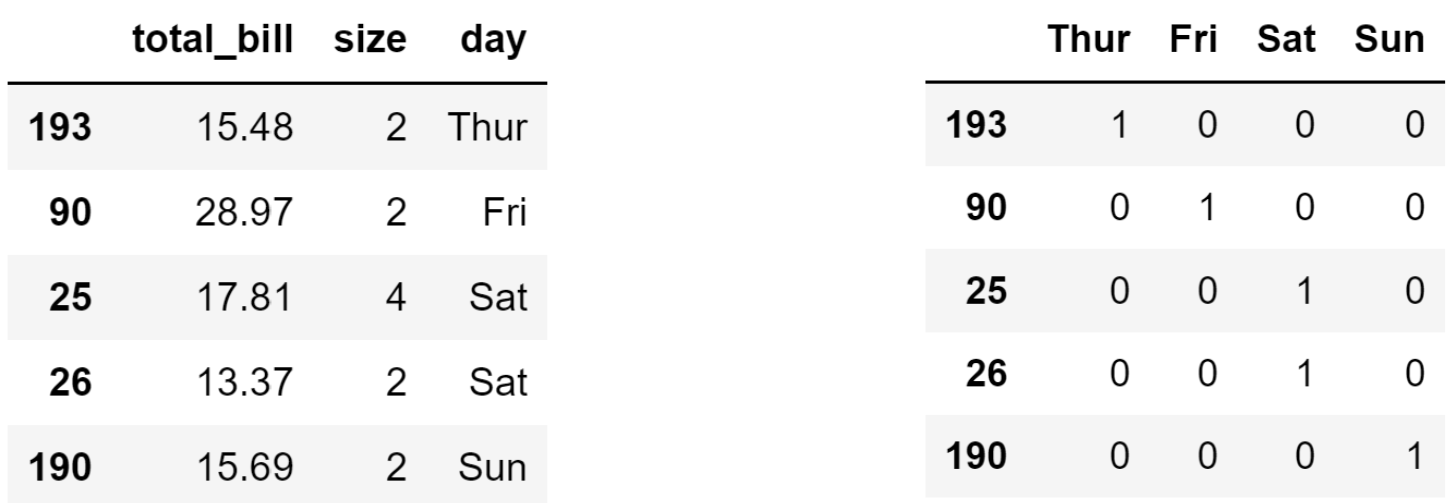
\includegraphics[scale=0.3]{figs/ln05/one-hot-encode.png}
    \end{center}
\end{ln-define}
Multiple Linear Regression, however, can suffer from this. \\
In our design matrix, we always have a column of $1$s: $\vec{1}$. \\
Using the exact example above, we can in fact find that:
\[\vec{Sunday} = \vec{1} - \vec{Thursday} - \vec{Friday} - \vec{Saturday}\]
because if a guest appeared on neither Thursday, Friday, nor Saturday, then the guest must appear on Sunday.
In this case, we have created a linearly dependent design matrix. \\
Fortunately, the Python library for one hot encoding has captured this deficiency, and provided remedy with optional arguments:
\setbox\codebox=\hbox{
    \begin{lstlisting}
    pd.get_dummies
    Args:
        data: A DataFrame, Series, or Array to One Hot Encode.
        drop_first: A boolean to indicate whether to drop the first 
        category of each categorical variable to encode, so to 
        prevent linear dependence.
    Returns:
        The result of One Hot Encoding data.
    \end{lstlisting}
}
\begin{ln-code}{One Hot Encoding via Pandas in Python}{}
    \usebox\codebox
\end{ln-code}
